%\documentclass[a4paper, 10pt, conference]{../../templates/IEEEconf/IEEEconf}
\documentclass[10pt, conference, onecolumn]{../../../templates/IEEEtran/IEEEtran}
%\documentclass[10pt, journal]{../../templates/IEEEtran/IEEEtran}

\usepackage{graphicx}
\usepackage{caption} 
\usepackage{subcaption}
\usepackage{hyperref}
\usepackage{listings}
\usepackage{hhline}
\usepackage{float}
\usepackage{amssymb}
\usepackage[autostyle=true]{csquotes}
\usepackage{amsmath}
\usepackage{marvosym}
\usepackage{minted}

\font\subtitlefont=cmr12 at 18pt

\title{First contact: Agents meet Haskell \\ {\huge Simulating epidemics using Functional Reactive Programming} \\ {\large An Agent-Based Approach}}

% IEEEtran journal authors
%\author{Jonathan Thaler, ̃Peer-Olaf Siebers \\ School of Computer Science \\ University of Nottingham%
%\thanks{jonathan.thaler@nottingham.ac.uk}%
%\thanks{peer-olaf.siebers@nottingham.ac.uk}
%}

% IEEEtran conference authors
\author{
	\IEEEauthorblockN{Jonathan Thaler}
	\IEEEauthorblockA{School of Computer Science\\
		University of Nottingham\\
		jonathan.thaler@nottingham.ac.uk}
		
	\and
		
	\IEEEauthorblockN{Thorsten Altenkirch}
	\IEEEauthorblockA{School of Computer Science\\
		University of Nottingham\\
		thorsten.altenkirch@nottingham.ac.uk}

	\and
	
	\IEEEauthorblockN{Peer-Olaf Siebers}
	\IEEEauthorblockA{School of Computer Science\\
		University of Nottingham\\
		peer-olaf.siebers@nottingham.ac.uk}
}

%\IEEEpubid{0000--0000/00\$00.00 ̃\copyright ̃2015 IEEE}

% IEEEconf authors
%\author{
%	Jonathan Thaler \\
%	\email{jonathan.thaler@nottingham.ac.uk} \\
%	\begin{affiliation}
%		School of Computer Science, University of Nottingham
%	\end{affiliation} \\
%	\and 
%	Peer-Olaf Siebers \\
%	\email{peer-olaf.siebers@nottingham.ac.uk} \\
%	\begin{affiliation}
%		School of Computer Science, University of Nottingham
%	\end{affiliation} 
%	\and 
%	Thorsten Altenkirch \\
%	\email{thorsten.altenkirch@nottingham.ac.uk} \\
%	\begin{affiliation}
%		School of Computer Science, University of Nottingham
%	\end{affiliation} 
%}

\begin{document}
\maketitle 

\begin{abstract}
TODO: cite my own 1st paper from SSC2017: add it to citations

TODO: refine it: start with simulating epidemics and then go into ABS

Agent-Based Simulation (ABS) is a methodology in which a system is simulated in a bottom-up approach by modelling the micro interactions of its constituting parts, called agents, out of which the global macro system behaviour emerges. So far, the Haskell community hasn't been much in contact with the community of ABS due to the latter's primary focus on the object-oriented programming paradigm. This paper tries to bridge the gap between those two communities by introducing the Haskell community to the concepts of ABS. We do this by deriving an agent-based implementation for the simple SIR model from epidemiology. In our approach we leverage the basic concepts of ABS with functional reactive programming from Yampa which results in a surprisingly fresh, powerful and convenient EDSL for formulating ABS in Haskell.
\end{abstract}

\begin{IEEEkeywords}
Functional Reactive Programming, Agent-Based Simulation
\end{IEEEkeywords}

\section{Introduction}
There exists a large number of simulation packages which allow the convenient creation of System Dynamics simulations by straight-forward visual diagram creation. One simply creates stocks and flows, connects them, specifies the flow-rates and initial parameters and then runs the model. An example for such a visual diagram creation in the simulation package AnyLogic can be seen in Figure \ref{fig:sir_stockflow_diagram}.

\begin{figure}
	\centering
	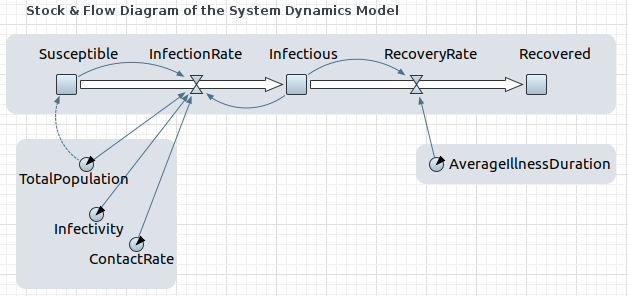
\includegraphics[width=.5\textwidth, angle=0]{./fig/SIR_SD_STOCKFLOW_DIAGRAMM.png}
	\caption{Visual System Dynamics Diagram of the SIR model in AnyLogic Personal Learning Edition 8.3.1.}
	\label{fig:sir_stockflow_diagram}
\end{figure}

Still, implementing System Dynamics directly in code is not as straight forward and involves numerical integration which can be quite tricky to get right. Thus, the aim of this paper is to look into how System Dynamics models can be implemented in code correctly without the use of a simulation package. We use the well known SIR model \cite{kermack_contribution_1927} from epidemiology to demonstrate our approach.

Our language of choice is Haskell because it emphasises a declarative programming style in which one describes \textit{what} instead of \textit{how} to compute. Further it allows to rule out interference with non-deterministic influences or side-effects already at compile-time. This is of fundamental importance for System Dynamics because it behaves completely deterministic and involves no stochastics or non-determinism whatsoever. Also, we make use of Functional Reactive Programming which allows to express continuous-time systems in a functional way. 

We show that by this approach we can arrive at correct-by-construction implementations of System Dynamic models. This means that the correctness of the code is obvious because we have closed the gap between the model specification and its implementation. Thus, the contribution of the paper is the demonstration of how to implement correct-by-construction System Dynamics simulations using Haskell and Functional Reactive Programming.

\section*{Acknowledgments}
The authors would like to thank I. Perez, H. Nilsson, J. Greensmith, T. Schwarz and H. Vollbrecht for constructive comments and valuable discussions.

\bibliographystyle{../../../templates/IEEEtran/bibtex/IEEEtran}
\bibliography{../../../../references/phdReferences.bib}

\appendices

\newpage
\section{Full code of the agent-based SIR implementation}
\label{app:abs_code}

\begin{minted}[fontsize=\footnotesize, linenos]{haskell}
data SIRState = Susceptible | Infected | Recovered deriving (Eq)
data SIRMsg = Contact SIRState deriving (Eq)

type SIRAgentState = SIRState

type SIREnvironment = [AgentId]

type SIRAgentDef = AgentDef SIRAgentState SIRMsg SIREnvironment
type SIRAgentBehaviour = AgentBehaviour SIRAgentState SIRMsg SIREnvironment
type SIRAgentBehaviourReadEnv = ReactiveBehaviourReadEnv SIRAgentState SIRMsg SIREnvironment
type SIRAgentBehaviourIgnoreEnv = ReactiveBehaviourIgnoreEnv SIRAgentState SIRMsg SIREnvironment
type SIRAgentIn = AgentIn SIRAgentState SIRMsg SIREnvironment
type SIRAgentOut = AgentOut SIRAgentState SIRMsg SIREnvironment
type SIRAgentObservable = AgentObservable SIRAgentState

type SIREventSource = EventSource SIRAgentState SIRMsg SIREnvironment

-------------------------------------------------------------------------------
infectivity :: Double
infectivity = 0.05

contactRate :: Double
contactRate = 5

illnessDuration :: Double
illnessDuration = 15

contactSS :: Int
contactSS = 20

illnessTimeoutSS :: Int
illnessTimeoutSS = 2

-------------------------------------------------------------------------------
createSIRNumInfected :: Int -> Int -> IO ([SIRAgentDef], SIREnvironment)
createSIRNumInfected agentCount numInfected = do
    let agentIds = [0 .. (agentCount-1)]
    let infectedIds = take numInfected agentIds
    let susceptibleIds = drop numInfected agentIds

    adefsSusceptible <- mapM (sirAgent Susceptible) susceptibleIds
    adefsInfected <- mapM (sirAgent Infected) infectedIds

    return (adefsSusceptible ++ adefsInfected, agentIds)

sirAgent :: SIRState -> AgentId -> IO SIRAgentDef
sirAgent initS aid = do
    rng <- newStdGen
    let beh = sirAgentBehaviour rng initS
    let adef = AgentDef { 
          adId = aid
        , adState = initS
        , adBeh = beh
        , adInitMessages = NoEvent
        , adConversation = Nothing
        , adRng = rng 
        }

    return adef
   
-------------------------------------------------------------------------------
-- UTILITIES
gotInfected :: SIRAgentIn -> Rand StdGen Bool
gotInfected ain = onMessageM gotInfectedAux ain False
  where
    gotInfectedAux :: Bool -> AgentMessage SIRMsg -> Rand StdGen Bool
    gotInfectedAux False (_, Contact Infected) = randomBoolM infectivity
    gotInfectedAux x _ = return x



respondToContactWith :: SIRState -> SIRAgentIn -> SIRAgentOut -> SIRAgentOut
respondToContactWith state ain ao = onMessage respondToContactWithAux ain ao
  where
    respondToContactWithAux :: AgentMessage SIRMsg -> SIRAgentOut -> SIRAgentOut
    respondToContactWithAux (senderId, Contact _) ao = sendMessage (senderId, Contact state) ao

-- SUSCEPTIBLE
sirAgentSuceptible :: RandomGen g => g -> SIRAgentBehaviour
sirAgentSuceptible g = 
	transitionOnEvent 
		sirAgentInfectedEvent 
		(readEnv $ sirAgentSusceptibleBehaviour g) 
		(sirAgentInfected g)

sirAgentInfectedEvent :: SIREventSource
sirAgentInfectedEvent = proc (ain, ao) -> do
    let (isInfected, ao') = agentRandom (gotInfected ain) ao 
    infectionEvent <- edge -< isInfected
    returnA -< (ao', infectionEvent)

sirAgentSusceptibleBehaviour :: RandomGen g => g -> SIRAgentBehaviourReadEnv
sirAgentSusceptibleBehaviour g = proc (ain, e) -> do
    ao' <- doOnce (setAgentState Susceptible) -< agentOutFromIn ain
    returnA -< sendMessageOccasionallySrcSS 
    			g
    			(1 / contactRate)
    			contactSS
    			(randomAgentIdMsgSource (Contact Susceptible) True) -< (ao', e)

-- INFECTED
sirAgentInfected :: RandomGen g => g -> SIRAgentBehaviour
sirAgentInfected g = 
	transitionAfterExpSS 
		g 
		illnessDuration 
		illnessTimeoutSS 
		(ignoreEnv $ sirAgentInfectedBehaviour g) 
		sirAgentRecovered

sirAgentInfectedBehaviour :: RandomGen g => g -> SIRAgentBehaviourIgnoreEnv
sirAgentInfectedBehaviour g = proc ain -> do
    ao' <- doOnce (setAgentState Infected) -< agentOutFromIn ain
    returnA -< respondToContactWith Infected ain ao'

-- RECOVERED
sirAgentRecovered :: SIRAgentBehaviour
sirAgentRecovered = doOnceR $ setAgentStateR Recovered

-- INITIAL CASES
sirAgentBehaviour :: RandomGen g => g -> SIRState -> SIRAgentBehaviour
sirAgentBehaviour g Susceptible = sirAgentSuceptible g
sirAgentBehaviour g Infected = sirAgentInfected g
sirAgentBehaviour _ Recovered = sirAgentRecovered

-------------------------------------------------------------------------------
runSIR :: IO ()
runSIR = do
    -- parallel strategy, no updating/folding of environment, no shuffling, rng-seed of 42
    params <- initSimulation Parallel Nothing Nothing False (Just 42)
    (initAdefs, initEnv) <- createSIRNumInfected agentCount numInfected
    let dynamics = simulateAggregateTime initAdefs initEnv params dt t aggregate
    print dynamics
	
aggregate :: (Time, [SIRAgentObservable], SIREnvironment) -> (Time, Double, Double, Double)
aggregate (t, aobs, _) = (t, susceptibleCount, infectedCount, recoveredCount)
  where
    susceptibleCount = fromIntegral $ length $ filter ((Susceptible==) . snd) aobs
    infectedCount = fromIntegral $ length $ filter ((Infected==) . snd) aobs
    recoveredCount = fromIntegral $ length $ filter ((Recovered==) . snd) aobs
\end{minted}

\end{document}